% arara: mkdir: { target: 'output' }
% arara: pdflatex: { options: ['-output-directory=output'] }
% arara: biber: { options: ['--wraplines', '--output-directory=output'] }
% arara: pdflatex: { options: ['-output-directory=output'] }
% arara: pdflatex: { options: ['-output-directory=output'] }
% arara: move: { files: [ 'output/main.pdf' ], target: 'Promillo.pdf' }
\documentclass[a4paper,12pt]{article}
\usepackage[T1]{fontenc} %% Umlaute
\usepackage[ngerman]{babel}
\usepackage[backend=biber, style=ieee]{biblatex}
\addbibresource{literatur.bib}
\usepackage{url}
\usepackage{float}
\usepackage{booktabs} % \usepackage{tabularx}
\usepackage[onehalfspacing]{setspace} %% Zeilenabstände, singlespacing 1-fach, onehalfspacing 1,5-fach, doublespacing 2-fach
\usepackage[format=plain,labelfont=bf]{caption}
\usepackage[left=3cm, right=2cm, top=3cm, bottom=3cm]{geometry}
\usepackage[hidelinks]{hyperref}
\usepackage{graphicx}
\usepackage{emptypage}
\usepackage[table]{xcolor}
\usepackage{minted}
\usepackage[autostyle=true]{csquotes} %mit \textquote Anführungszeichen
\definecolor{codegreen}{rgb}{0,0.6,0}
\definecolor{codegray}{rgb}{0.5,0.5,0.5}
\definecolor{codepurple}{rgb}{0.58,0,0.82}
\definecolor{backcolour}{rgb}{0.95,0.95,0.92}

\usepackage{fancyhdr} % Kopf/Fußzeile
\usepackage[parfill]{parskip}

\newcommand{\changefont}{\fontsize{7}{12}\selectfont}
\newcommand{\changefontbig}{\fontsize{10}{12}\selectfont}

\setcounter{biburllcpenalty}{9000}% Kleinbuchstaben
\setcounter{biburlucpenalty}{9000}% Großbuchstaben
\widowpenalty = 4500
\clubpenalty = 4500% Vermeidung von Absatzende auf nöchster Seite

\renewcommand{\listingscaption}{Quellcode}%

%%Neudefinition Autoref
\addto\extrasngerman{%
    \def \listingautorefname{\listingscaption}%
}%

\renewcommand*{\maketitle}{%

	% Vorlage für WABs der Provadis Hochschule
	% basiert auf "Universität Ulm Praktikumsbericht Vorlage"
	% von Max Sch.
	% CC BY 4.0
	%
	% Titelseite.tex
	%
	% Hier wird die Titelseite erzeugt.


	\begin{titlepage}

		% Logo Provadis Hochschule und ggf. Logo Arbeitgeber
		
\includegraphics[height=2.06cm]{images/provadis-hochschule.pdf}
		\hfill

		\vspace*{1cm}

		\begin{singlespace}
			\begin{center}

				\normalsize
				Cookbook

				\vspace*{2cm}

				\large

				\textbf{Promillo}

				\vspace*{3cm}

				Für das Modul New Trends in IT und Management der digitalen Transformation\\
				Provadis School of International Management and Technology\\
				von

				\vspace*{1.5cm}

				Ole Grundmann \\
                Moritz Bosch \\
                Ben Zelleröhr \\

                \normalsize
                \vfill % variabler vertikaler Abstand
                \begin{tabular}{@{}ll}
                    ole.grundmann@stud-provadis-hochschule.de  & D493 \\
                    moritz.bosch@stud-provadis-hochschule.de   & D490 \\
                    ben.zelleroehr@stud-provadis-hochschule.de & D532 \\
                \end{tabular}

			\end{center}
		\end{singlespace}


	\end{titlepage}

	% Ende der Datei
}


\begin{document}
\maketitle
\setcounter{page}{2}
\pagestyle{fancy}
\fancyhf{}

%% Nices Design
\setlength{\headheight}{18pt}
\fancyhead[L]{\changefontbig\nouppercase{\textit{\leftmark}}}
\fancyhead[R]{\changefontbig\thepage}

\cleardoublepage
\tableofcontents

\cleardoublepage
\section{Einleitung}\label{sec:einleitung} % (fold)

% section Einleitung (end)


% \clearpage
% \input{sec/02-forschungs-stand}

\clearpage
\section{Cook}\label{sec:cook} % (fold)

Für die Reproduktion des Workflows mit identischer Einrichtung werden zwei Programme benötigt: nginx
als Reverse Proxy sowie Docker zur Ausführung des n8n-Containers und der MongoDB-Datenbank.


Im bereitgestellten ZIP-Archiv befindet sich die Datei \verb|nginx.conf|. In dieser Datei ist in Zeile 4
und in Zeile 13 der korrekte Domainname einzutragen. In Zeile 10 und in Zeile 11 sind der Pfad zum
SSL-Zertifikat und der Pfad zum zugehörigen privaten Schlüssel anzupassen. Nach der Anpassung wird
die Datei in das Verzeichnis \verb|/etc/nginx/sites-available| kopiert und mit einem aussagekräftigen
Namen, beispielsweise n8n, versehen. Anschließend wird im Verzeichnis
\verb|/etc/nginx/sites-enabled| ein
symbolischer Link auf die Konfigurationsdatei erstellt:

\begin{verbatim}
ln -s /etc/nginx/sites-available/n8n /etc/nginx/sites-enabled/n8n
\end{verbatim}

Damit die Änderungen wirksam werden, ist der nginx-Dienst neu zu laden:

\begin{verbatim}
nginx -s reload
\end{verbatim}

Im entpackten ZIP-Archiv befindet sich ebenfalls die Datei \verb|.env.example|. Diese ist in
\verb|.env| umzubenennen. In der Datei wird der Domainname eingetragen. Der Start von n8n und
MongoDB erfolgt über den folgenden Befehl:

\begin{verbatim}
docker compose up
\end{verbatim}

Standardmäßig wird dabei die aktuelle stabile Version von n8n verwendet. Die gewünschte Version kann
in der Datei \verb|docker-compose.yml| festgelegt werden. Die zuletzt getestete Version ist
\verb|1.105.3|.

Beim ersten Aufruf des n8n-Servers wird die Erstellung eines Benutzerkontos abgefragt. Nach
erfolgreichem Abschluss der Registrierung erfolgt die Weiterleitung zur Übersichtsseite, die
\autoref{fig:n8n_overview} dargestellt ist.

\begin{figure}
    \begin{center}
        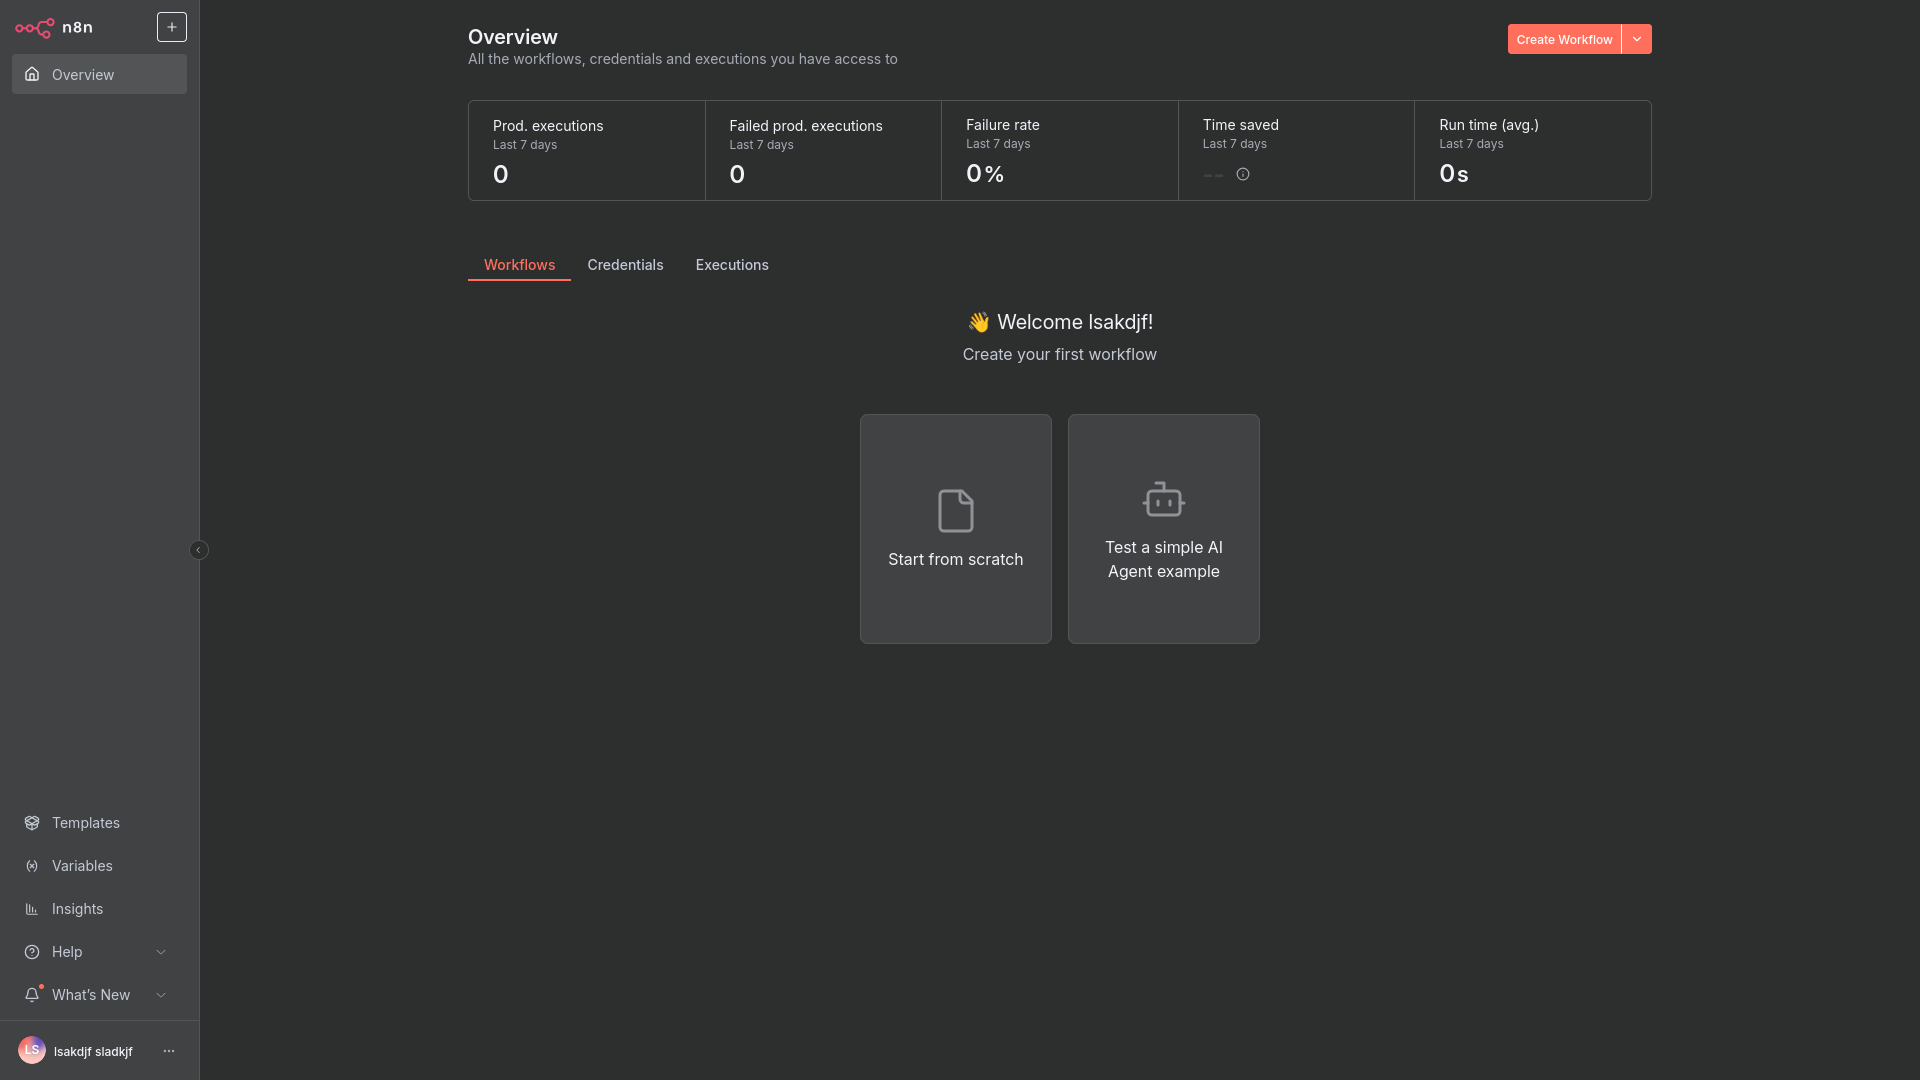
\includegraphics[width=0.95\textwidth]{images/n8n_overview.png}
    \end{center}
    \caption{n8n Übersichtsseite}\label{fig:n8n_overview}
\end{figure}

% section Cook (end)


\cleardoublepage
\printbibliography[heading=bibintoc, title={Literaturverzeichnis}]

\end{document}
